% \begin{figure}
%     \centering
%     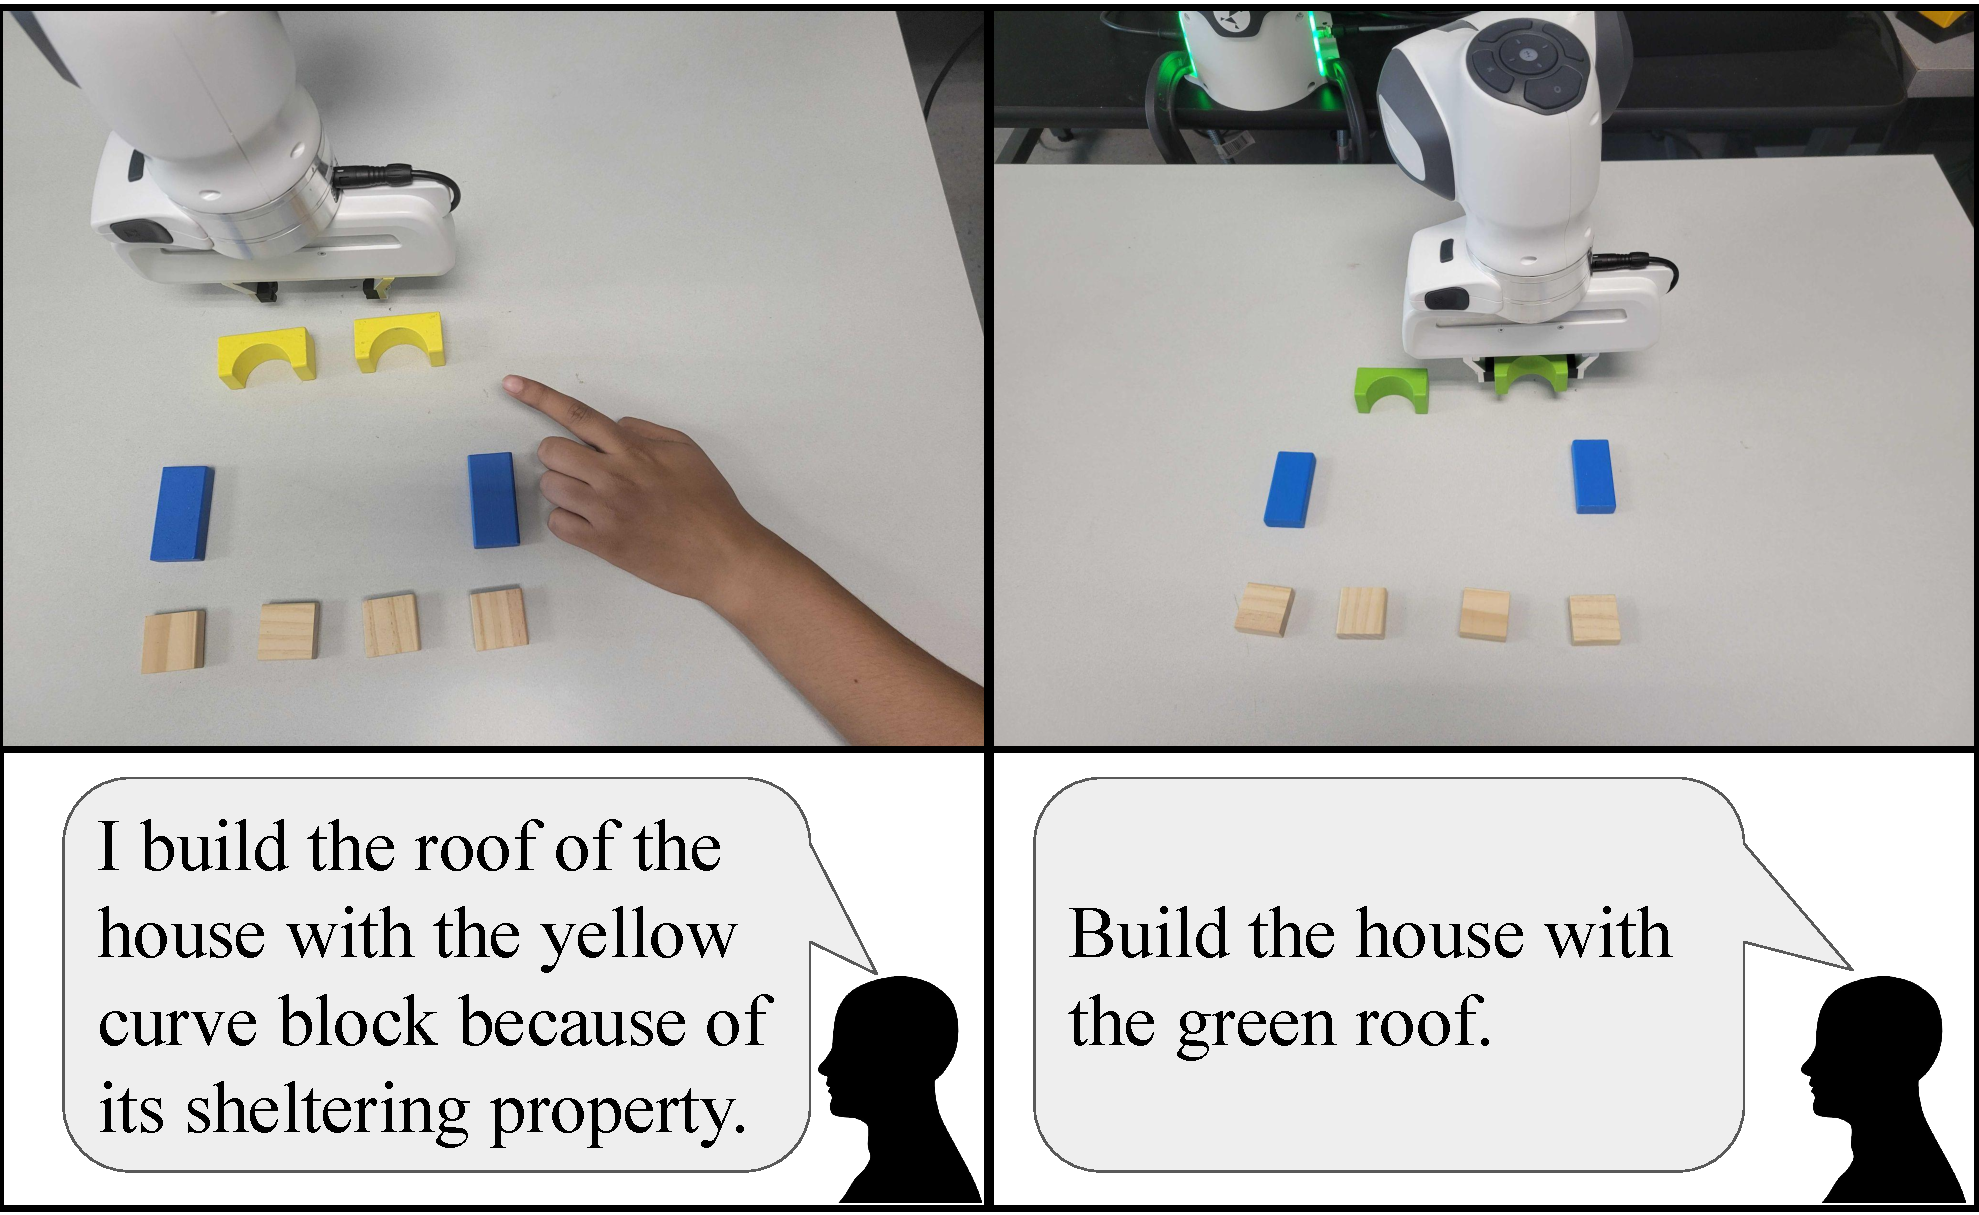
\includegraphics[width=\linewidth]{figures/figure1_2grid.pdf}
%     \caption{A figure that demonstrate how our concept net model represents the knowledge graph.}
%     \label{fig:concept_net_model}
%     \vspace{-5mm}
% \end{figure}


% \begin{figure*}
%     \centering
%     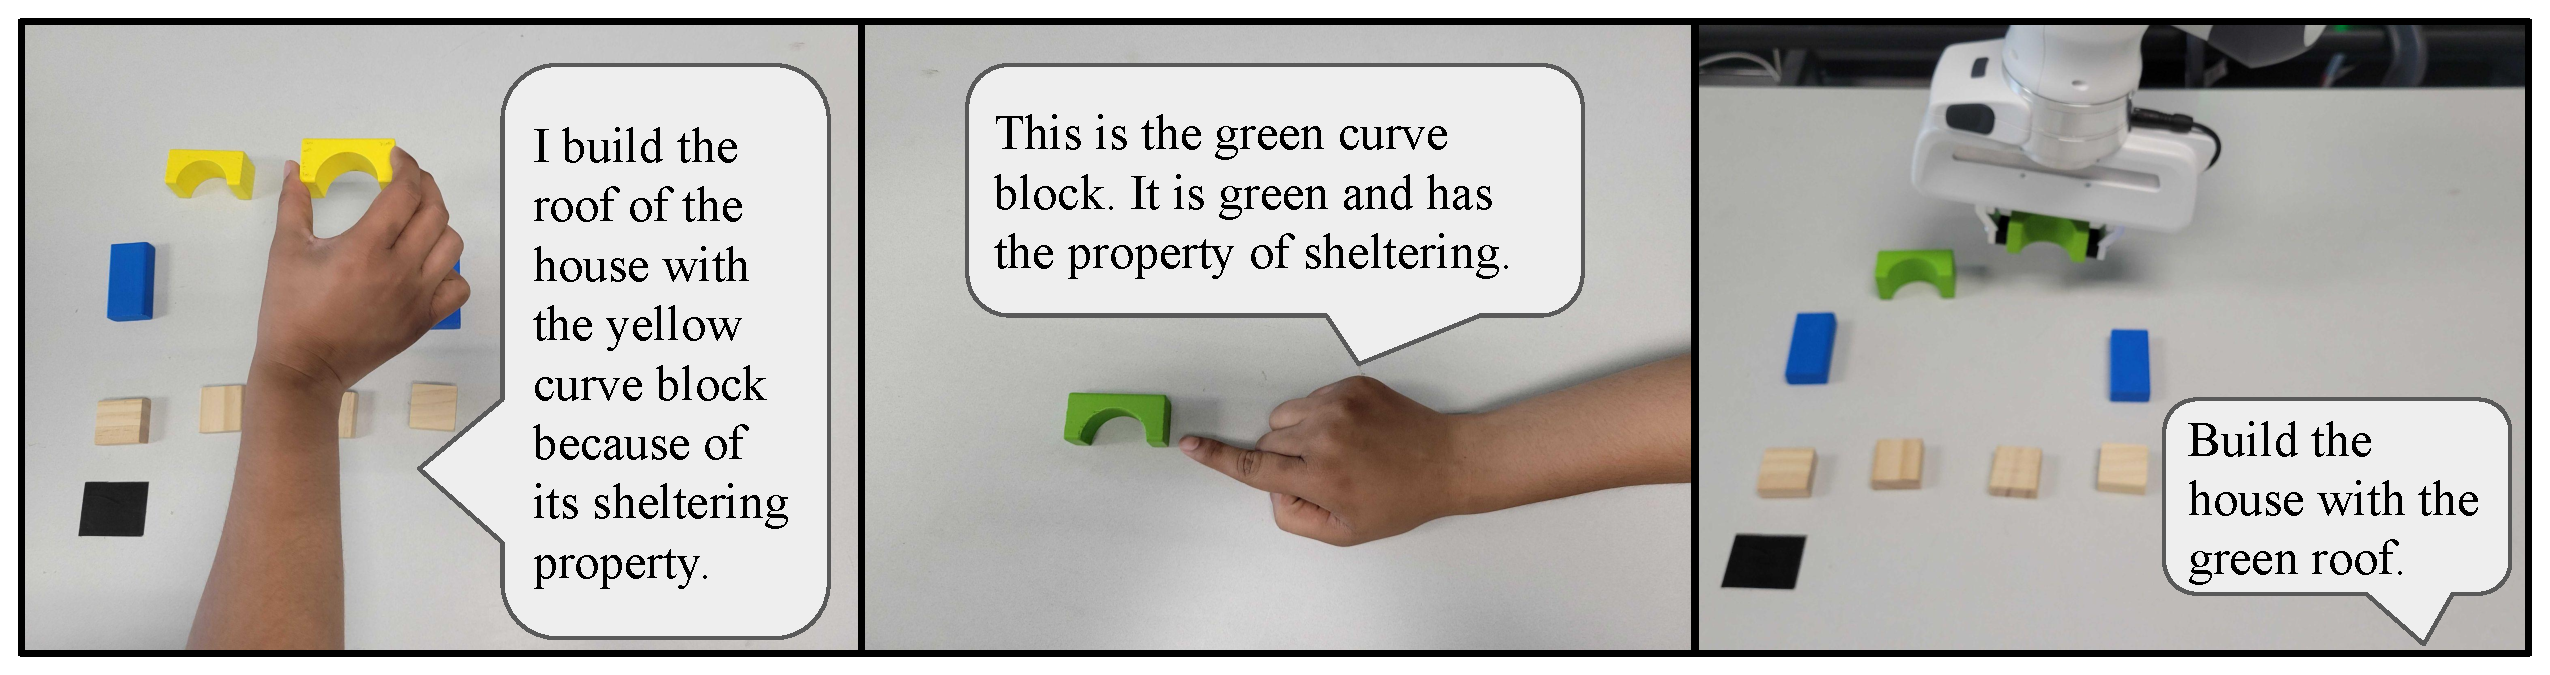
\includegraphics[width=0.8\textwidth]{figures/figure1_3grid.pdf}
%     \caption{This figure demonstrates how Hi-Viscont learns from users interactively. (a) First the user demonstrates a structure, say a ``house,'' with its sub-components such as its ``roof'' and the concepts used to make the ``roof'' such as a ``curved block''. (b) The user then teaches a novel concept such as a ``green curved block'' and describes its properties. (c) The user can now ask the robot to create a new structure (``house with green roof'') zero-shot with the taught component without explicitly asking for the object of interest. Our model uses a combination of pre-trained visual features, and a Graph Neural Network backbone to update concepts taught and their ancestors to help the robot in continual learning settings such as the domain demonstrated.}
%     \label{fig:interactive_task_teaching}
%     \vspace{-5mm}
% \end{figure*}

\begin{figure*}[h]
  \centering
\begin{subfigure}{0.28\textwidth}
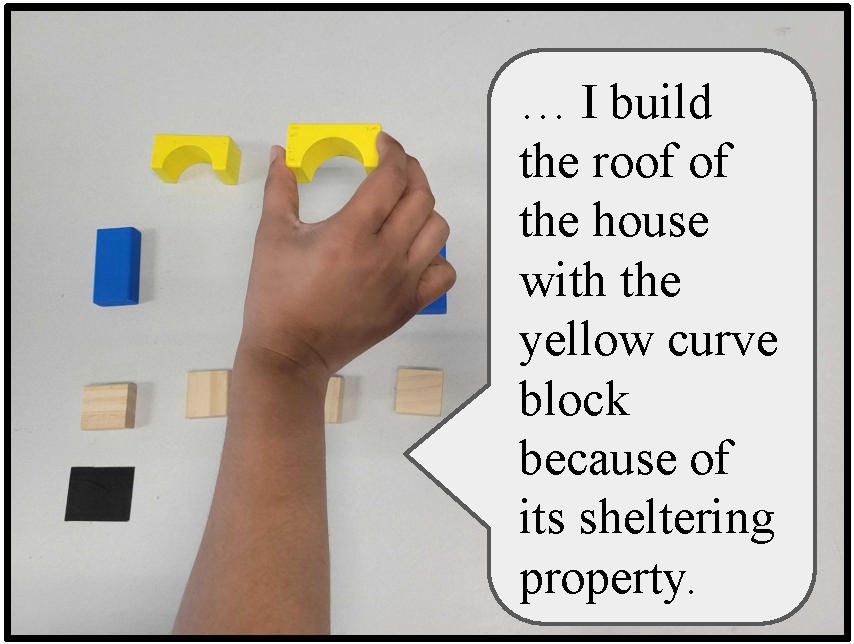
\includegraphics[width=\textwidth,page=1]{figures/figure1_breakdown.pdf}
  \subcaption{}
\end{subfigure}
\hspace{0.01\textwidth}
% <— this is important. There should be no empty line here. 
\begin{subfigure}{0.28\textwidth}
\includegraphics[width=\textwidth,page=2]{figures/figure1_breakdown.pdf}
  \subcaption{}
\end{subfigure}
\hspace{0.01\textwidth}
%
\begin{subfigure}{0.28\textwidth}
\includegraphics[width=\textwidth,page=3]{figures/figure1_breakdown.pdf}
  \subcaption{}
\end{subfigure}


\caption{This figure demonstrates how Hi-Viscont learns from users interactively. (a) First, the user demonstrates a structure, say a ``house,'' with its sub-components such as a ``roof'' and the concepts used to make the ``roof'' such as a ``yellow curve block''. (b) The user then teaches a novel concept such as a ``green curve block'' and describes its properties. (c) The user can now ask the robot to create a new structure (``house with green roof'') zero-shot with the taught component without explicitly asking for the object of interest. }
%Our model uses a combination of pre-trained visual features, and a Graph Neural Network backbone to update concepts taught and their ancestors to help the robot in continual learning settings such as the domain demonstrated}
\label{fig:interactive_task_teaching}
\end{figure*}


% What's the problem we are solving?
% 1. learning task interactively
% 2. learning novel concept interactively
% 3. generalize to unseen task 
% Need figure 1.
Robots in a household will encounter novel objects and tasks all the time. For example, a robot might need to use a novel vegetable peeler to peel potatoes even though it has never seen, let alone used such a peeler before. Our work focuses on teaching robots novel concepts and tasks one-shot via human-robot interactions,
% We want to teach task interactively to a robot along with novel concepts. 
% For such learning on the robot we want to enable 
% We aim to teach visual tasks to robot via natural interactions with a human teacher 
which include demonstrations and linguistic explanations.
% , which include seeing human demonstrating the task and listening to the human describe the task. 
We then want the robot to generalize to a similar but unseen visual task. 
% Additionally, the robot should be able to learn more concepts to perform more variants of tasks. 
% In this work we present a neuro-symbolic approach to learn generalizable visual tasks and concepts from human interactions as demonstrated in Fig.~\ref{fig:interactive_task_teaching}.  
A robotic system that can learn generalizable tasks and concepts from few natural interactions from a human-teacher would represent a large leap for robotics applications in everyday settings. 
In this work we aim to take a step in the direction of generalizable interactive learning as demonstrated Fig.~\ref{fig:interactive_task_teaching}. 

% SoTA
% Prior works
% why the prior work does not resolve these problems
% LLM methods
Previously, large image and language models have been extended to robotics to manipulate novel objects, and create visual scenes~\citep{shridhar2021cliport, brohan2023rt2}. 
These methods recognize novel objects by using their underlying large language and visual models to extract task-relevant knowledge.
However, they are not capable of learning to create a novel visual scene from  in-situ interactions with a human user.
There is also significant work in few-shot learning of  visual concepts in computer vision~\citep{mei2022falcon, snell2017prototypical,vinyals2017matching, sung2018learning, wang2018zeroshot, tian2020rethinking}, albeit without extensions to robotics domains.
% \asnote{Is the introduction of the reverse path a bit abrupt?}
These approaches focus on learning novel concepts for image classification, but ignore the fact that the novel concepts also bring new information to update our understanding of concepts already known to the robot.
% Some of these works improved the representation of the new concepts by propagating knowledge from related known parent concepts\cite{mei2022falcon, wang2018zeroshot, kampffmeyer2019rethinking}, but ignored the knowledge propagation in the opposite direction from child to parent.
The reverse path of knowledge propagation, that is, from novel concepts to previously known concepts is equivalently important in performing tasks in the real-life scenarios, especially when the agent has little knowledge of the world and needs to continually add information to known concepts. 
% This is because this type of knowledge propagation can help the agent to augment the general property of known objects continually, and therefore enable agents to utilize similar objects to solve novel tasks. Our focus is on these settings where the robot learns novel concepts and tasks and can generalize to solve novel permutations of these concepts and tasks.
% On the other hand, there are many works that robot learn to execute tasks following language request
% These method are also not capable to learn a novel task, or a novel concept via an in-situ demonstration.


% Our idea
%In this work, we propose a novel framework that enable the robot to learn visual task and visual concepts from natural interaction with human.
%Furthermore, our framework enables the agent to generalize to unseen variants of the taught visual tasks utilizing its knowledge
In this work, we propose a novel framework, Hi-Viscont, that enables robots to learn visual tasks and visual concepts from natural interactions with a human user. We learn the task type and concepts from users one-shot, and then generalize to novel task variants within the task type zero-shot.  
We do this by connecting our insights on \emph{one-shot visual concept learning} and the use of \emph{scene graphs}. 
% Previously scene graphs have been used for semantic mapping within robotics. 
% \asnote{Can we add any sort of punctuation to make to add a break to the following sentence.}T
The robot learns the structure of a visual task by converting linguistic interactions with a human user into a scene graph with language annotations. 
Moreover, Hi-Viscont updates parental concepts of the novel concept being taught. Such updates allow us to generalize the use of the novel concepts in to solve novel tasks.
% \asnote{We have used Hi-Viscout twice consecutively is that fine?}
% Hi-Viscont improves upon the existing state-of-the-art concept learning frameworks by introducing an additional module that updates the representations of all the related concepts. 


% Results
% \wgnote{Do we need this line here? This seems very much the same as the contribution paragraph}
% We present SOTA results in one-shot concept learning, a completely novel framework to solve visual tasks on the robot, and a human-subjects experiment demonstrating the use of our robot learning algorithm with real users. 

% Our proposed framework achieves a higher performance in visual question answering compared to the State-of-the-art one-shot concept learning framework FALCON\cite{mei2022falcon}.
% This is true for objective metric,
% waiting for Anant to send me the comparison survey
% Additionally, our framework achieves a better performance in all metrics of our human subject study with significance.
% 
% standardize paragraph
The contribution of this work is three-fold:
\begin{enumerate}[noitemsep,topsep=0pt,parsep=0pt,partopsep=0pt]
    \item We present concept learning results on VQA tasks that are comparable to the state-of-the-art FALCON model. More specifically, Hi-Viscont improves on FALCON on all non-leaf concepts across all domains with significance.
    %\item We present SOTA visual concept learning results on VQA. We improve visual concept learning frameworks by continually updating the knowledge base for all concepts. 
    % This update creates a more robust framework for continual learning with  zero-shot generalization to unseen tasks. 
    %Hi-Viscont improves from FALCON by an average of $5.4\%$ across our three datasets.
    %Hi-Viscont improves the f1 score from the baseline model by at least $1.7\%$ in each of the three domains on VQA with significance
    %. \ngnote{averaged results here!}
    \item We enable the robot agent to learn a visual task from in-situ interactions with a scene graph, allowing zero-shot generalization to an unseen task of the same type, as demonstrated in Fig.~\ref{fig:interactive_task_teaching}. 
    % The robot agent can restore the structure of the demonstrated visual task with any object recognition algorithm.
    \item Finally, we conduct a human-subjects experiment to show that our system is able to learn visual tasks and concepts from in-situ interactions with human users. Hi-Viscont achieves a $33.33\%$ improvement in Success Rate when completing the users' requests compared to FALCON ($p=0.014$).
    
\end{enumerate}
